% Standalone TikZ architecture diagram for the paper
% Compile with: pdflatex architecture.tex
\documentclass[tikz,border=2pt]{standalone}
\usepackage{tikz}
\usetikzlibrary{arrows.meta,positioning,fit,calc,backgrounds}
\usepackage{amsmath}

\definecolor{graphblue}{RGB}{41,128,185}
\definecolor{sageorange}{RGB}{230,126,34}
\definecolor{gatpurple}{RGB}{142,68,173}
\definecolor{decodergreen}{RGB}{39,174,96}
\definecolor{bochnerred}{RGB}{192,57,43}
\definecolor{lightgray}{RGB}{245,245,245}

\begin{document}
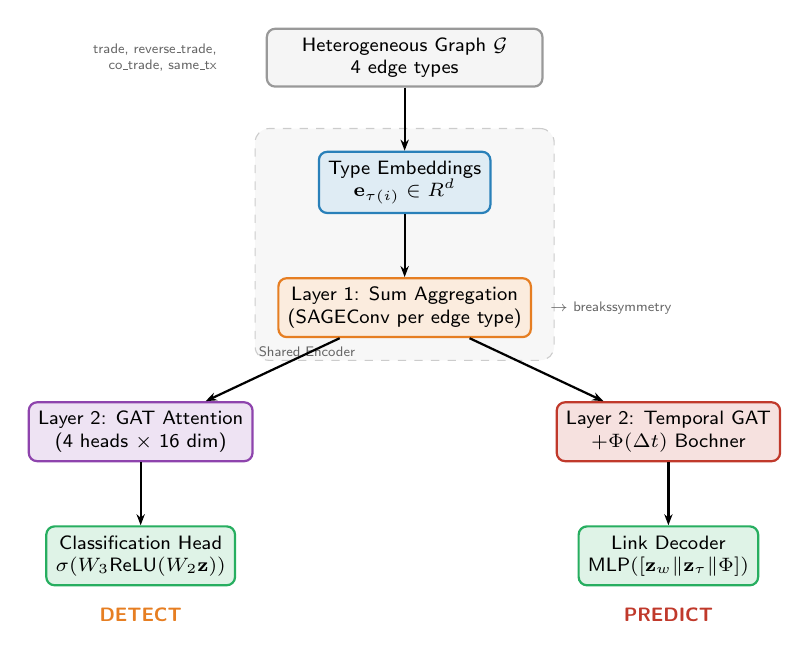
\begin{tikzpicture}[
    node distance=0.6cm and 0.8cm,
    block/.style={draw, rounded corners=3pt, minimum width=2.0cm,
                  minimum height=0.7cm, font=\scriptsize\sffamily,
                  align=center, thick},
    arrow/.style={-{Stealth[length=4pt]}, thick},
    label/.style={font=\tiny\sffamily, text=black!60},
]

% --- Input layer ---
\node[block, fill=graphblue!15, draw=graphblue]
    (embed) {Type Embeddings\\$\mathbf{e}_{\tau(i)} \in \mathbb{R}^{d}$};

% --- Layer 1 ---
\node[block, fill=sageorange!15, draw=sageorange, below=0.8cm of embed]
    (sage) {Layer 1: Sum Aggregation\\(SAGEConv per edge type)};

\node[label, right=0.1cm of sage] {$\to$ breaks\\symmetry};

% --- Layer 2 splits ---
\node[block, fill=gatpurple!15, draw=gatpurple,
      below left=0.8cm and 0.3cm of sage]
    (gat) {Layer 2: GAT Attention\\(4 heads $\times$ 16 dim)};

\node[block, fill=bochnerred!15, draw=bochnerred,
      below right=0.8cm and 0.3cm of sage]
    (tgat) {Layer 2: Temporal GAT\\$+ \Phi(\Delta t)$ Bochner};

% --- Outputs ---
\node[block, fill=decodergreen!15, draw=decodergreen,
      below=0.8cm of gat]
    (cls) {Classification Head\\$\sigma(W_3 \text{ReLU}(W_2 \mathbf{z}))$};

\node[block, fill=decodergreen!15, draw=decodergreen,
      below=0.8cm of tgat]
    (link) {Link Decoder\\$\text{MLP}([\mathbf{z}_w \| \mathbf{z}_\tau \| \Phi])$};

% --- Task labels ---
\node[font=\scriptsize\bfseries\sffamily, below=0.15cm of cls, text=sageorange]
    {DETECT};
\node[font=\scriptsize\bfseries\sffamily, below=0.15cm of link, text=bochnerred]
    {PREDICT};

% --- Arrows ---
\draw[arrow] (embed) -- (sage);
\draw[arrow] (sage) -- (gat);
\draw[arrow] (sage) -- (tgat);
\draw[arrow] (gat) -- (cls);
\draw[arrow] (tgat) -- (link);

% --- Graph input ---
\node[block, fill=lightgray, draw=black!40,
      above=0.8cm of embed, minimum width=3.5cm]
    (graph) {Heterogeneous Graph $\mathcal{G}$\\4 edge types};

\draw[arrow] (graph) -- (embed);

% --- Edge type annotations ---
\node[label, left=0.5cm of graph, text width=2.2cm, align=right]
    {trade, reverse\_trade,\\co\_trade, same\_tx};

% --- Shared encoder box ---
\begin{scope}[on background layer]
    \node[draw=black!20, dashed, rounded corners=5pt,
          fill=black!3, inner sep=8pt,
          fit=(embed)(sage)] (encoder) {};
    \node[label, above right=-2pt and -2pt of encoder.south west]
        {Shared Encoder};
\end{scope}

\end{tikzpicture}
\end{document}
